\section{Asymmetric Encryption}

In a Asymmetric encryption algorithm, there are a pair of keys. A public key that is available to everyone and therefore is \textbf{not a secret}, and a private key, that is only known to one user. The message encrypted with the public key only can be read with the private key, and with only the public key, it is impossible to know the private key. This allows us to create a system where everyone can send messages securely to a entity, but only the one with the private key can know its content.
This can work the other way around. The owner of the private key can cipher a message with it and send it to everyone. Then all the receivers can decipher the message with the public key. This may seem useless because everyone has the public key and is able to read the message. The interesting part is that only somebody that has the public key can create a message that can be read using the public key, so this way the message can be authenticated. This property in combination with the hash function, is very used in authentications and digital signatures.

Is worth mentioning that public key cryptography is generally more computationally expensive than symmetric cryptography. Usually the protocols use public key cryptography to authenticate and to exchange symmetric keys, then the rest of the communication is done using symmetric cryptography.
 
\begin{figure}[htb]
	\begin{centering}
		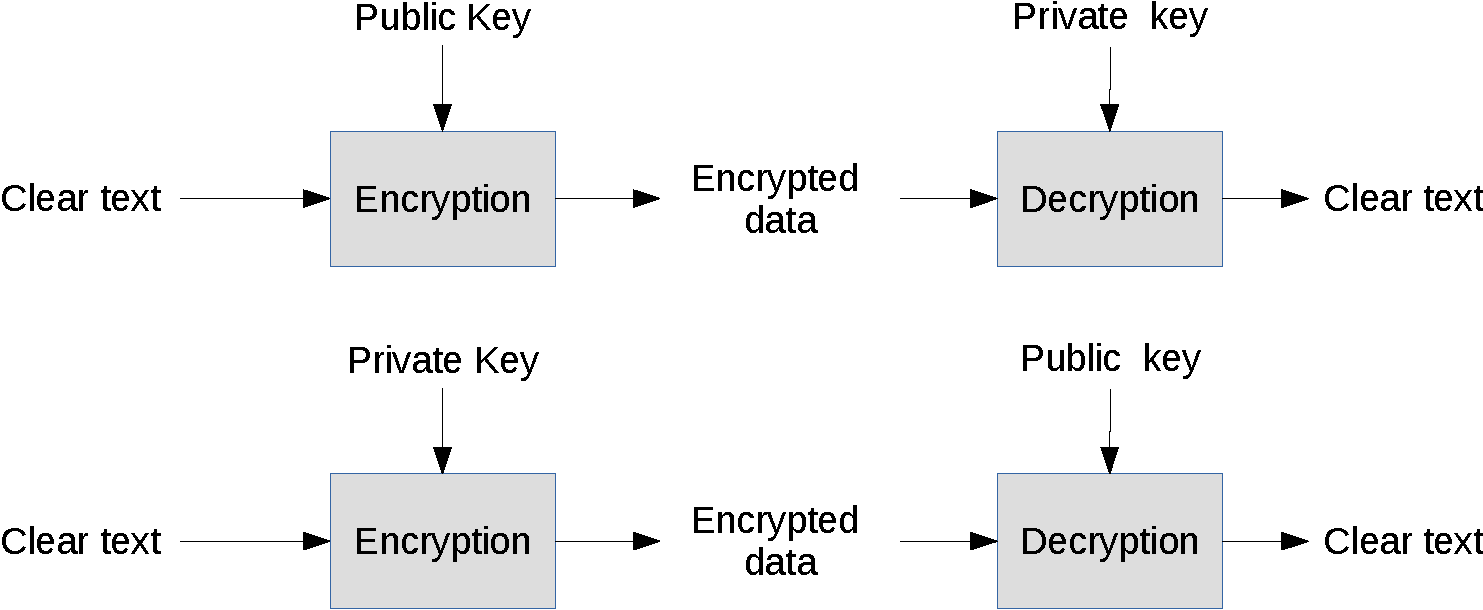
\includegraphics[width=0.7\columnwidth]{\securitydir/basicJsCrypto/figures/rsa}
		\par\end{centering}
	\caption{\label{fig:rsa} RSA can be used both ways}
\end{figure}